\documentclass[a4paper,12pt]{article}
\usepackage[a4paper, margin=2.4cm]{geometry}
\usepackage[utf8]{inputenc}
\usepackage{amsmath, amssymb} % Packages pour les maths
\usepackage[T1]{fontenc}
\usepackage{graphicx} 
\usepackage{caption}
\usepackage{setspace} % Espacement des lignes
\usepackage{tikz}
\usetikzlibrary{patterns}
\usepackage{hyperref}
\usepackage{titlesec}
\titleformat*{\section}{\LARGE\bfseries}
\titleformat*{\subsection}{\Large\bfseries}
\titleformat*{\subsubsection}{\normalsize\bfseries}
\begin{document}
\section*{Modèle 4: }
\subsubsection*{Hypothèses:}
\begin{itemize}
    \item Terre modélisée avec les continents, les mers, les océans 
    \item  On néglige: 
    \begin{itemize}
        \item convection dans l'air
        \item la conduction entre centre de la terre et croûte
        \item la conduction entre croûte et air (\(P_{th,cond}\))
    \end{itemize} 
    \item  rayonnement de la croûte (\(P_{th,ray}\))
    \item On considère la température de l'atmosphère constante dans l'espace et  au cours du temps 
    \item On prend en compte l'albédo du sol en fonction de la position et du mois de l'année 
    \item On prend en compte l'albedo des nuages.
    \item la capacité thermique dépend de la localisation
    \item On considère $T(t=0) = T_i$ \  indépendant de l'espace  
    \item On prend en compte la chaleur latente considérée avec des constantes propres à chaque continent\\
    
    
    
    
\end{itemize}

\subsubsection*{Schéma:} 
\noindent\textcolor{gray}{\rule{\linewidth}{0.4pt}}

    
\begin{center}
  \input{modele4/figures/Schéma modèle 4.txt }
\end{center}
\noindent\textcolor{gray}{\rule{\linewidth}{0.4pt}}
\vspace{0.2cm}
\subsubsection*{Équations de transfert thermique}

On applique le premier principe appliqué au système \{ Un pavé de hauteur h, de surface S de la Terre \}
\ \ 
\[
C \frac{dT}{dt} =(1-A_1)(1-A_2)\phi-\sigma T^4+\sigma T_{atm}^4-\fracQ_{lat}
\]
Avec \(C\) la capacité thermique surfacique en \(J\cdot K^{-1}\cdot m^{-2}\)

\vspace{0.5cm}
\subsubsection*{Calculs capacités calorifiques en fonction de la composition des surfaces}
Données récoltées sur : 
\url{https://data.catds.fr/cpdc/Land_products/GRIDDED/L4SM/OPER/}

\begin{itemize}
    \item Moyenne faite sur une période de 1 an grâce à 12 données récoltés le matin et 12 données récoltés le soir 
    \item Les 12 données ont été prise à des périodes différentes sur l'année 
    \item La masse volumique de la Terre est approximée constante 
\end{itemize}
\[
w = \frac{\rho_w \theta}{\rho_b (1 - \theta) + \rho_w \theta}
\]
Avec \(\theta\): le taux d'humidité en \(m^3\) d'eau par \(m^3\) de sol 
\[
c_p = c_{p,\text{sec}} + w (c_{p,\text{eau}} - c_{p,\text{sec}})
\]
Avec \(w\): la fraction massique d'eau 
\begin{table}[h!]
\centering
\begin{tabular}{ll}
\textbf{Constante} & \textbf{Valeur} \\
\hline
$c_{p,\text{sec}}$ & \SI{0.80}{\kilo\joule\per\kilogram\per\kelvin} \\
$c_{p,\text{eau}}$ & \SI{4.187}{\kilo\joule\per\kilogram\per\kelvin} \\
$\rho_b$ (sol) & \SI{1300}{\kilogram\per\cubic\metre} \\
$\rho_w$ (eau) & \SI{1000}{\kilogram\per\cubic\metre} \\
\end{tabular}
\caption*{Constantes utilisées pour le calcul de $c_p$}
\vspace{1cm}
\end{table}

\subsubsection*{Modélisation graphique (à Paris) :} 
\begin{itemize}
    \item Modèle adaptatif
\end{itemize}

\begin{center}
  \includegraphics[width=0.8\linewidth]{modele4/figures/adaptatif_année.jpeg}
  \end{center}
\begin{center}
  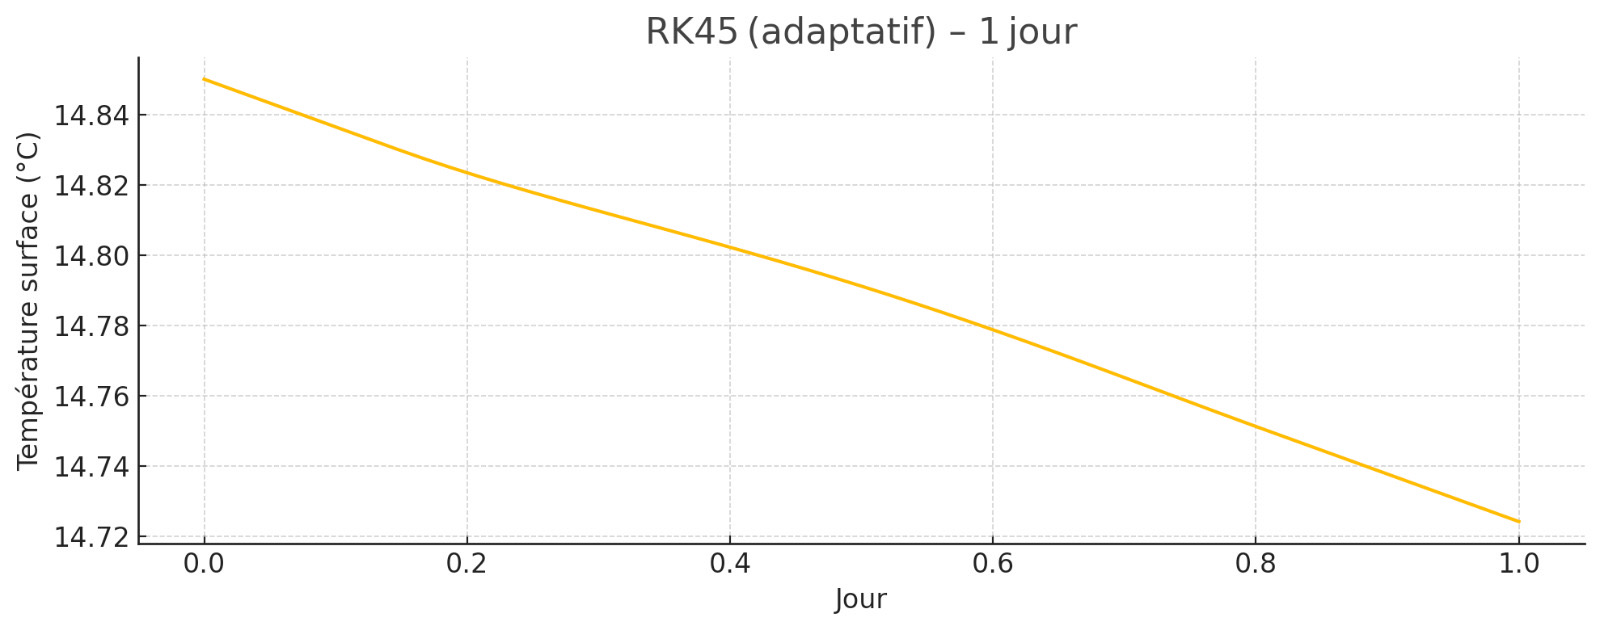
\includegraphics[width=0.8\linewidth]{modele4/figures/adaptatif_jour.jpeg}
  \end{center}
\begin{itemize}
    \item Modèle explicite
\end{itemize}


\begin{center}
  \includegraphics[width=0.8\linewidth]{modele4/figures/explicite_année.jpeg}
  \end{center}
\begin{center}
  \includegraphics[width=0.8\linewidth]{modele4/figures/explicité_jour.jpeg}
  \end{center}
\begin{itemize}
    \item Modèle réccurent
\end{itemize}

\begin{center}
  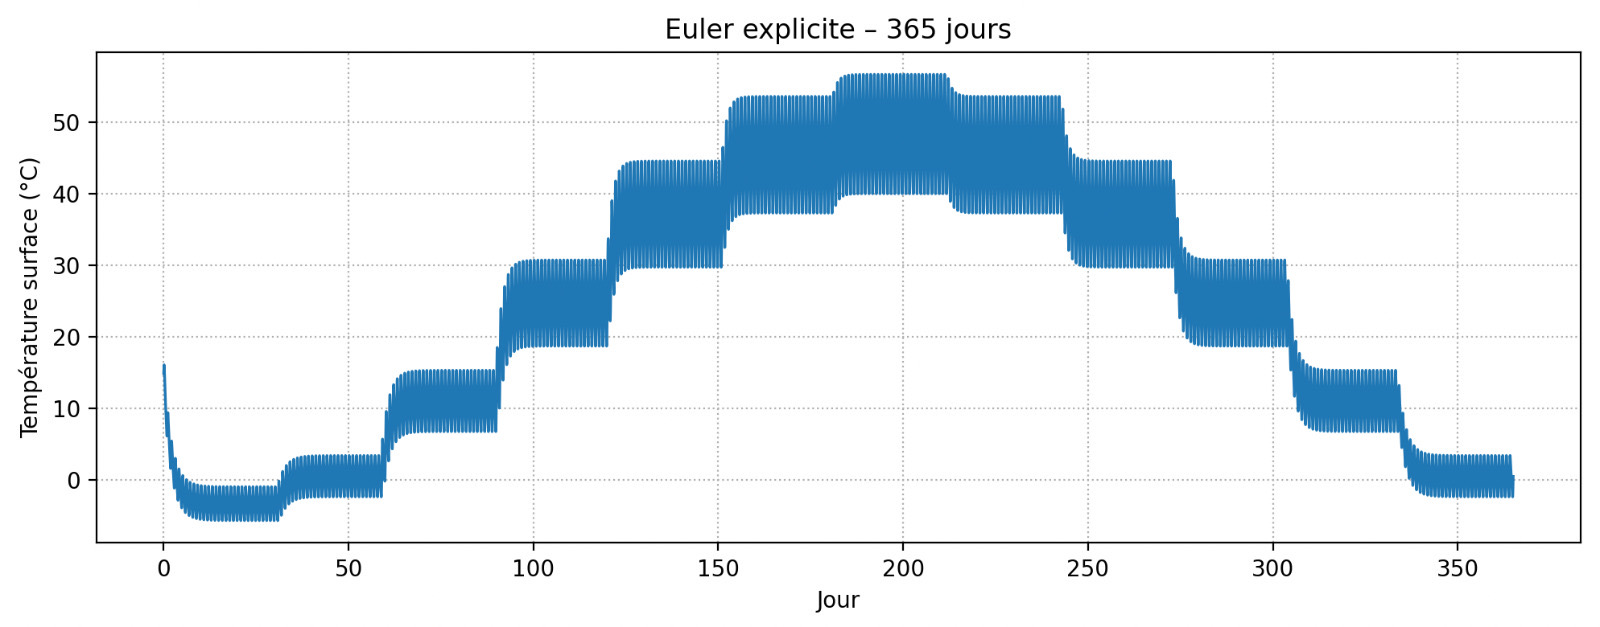
\includegraphics[width=0.8\linewidth]{modele4/figures/récurrent_année.jpeg}
  \end{center}
\begin{center}
  \includegraphics[width=0.8\linewidth]{modele4/figures/récurent_jour.jpeg}
  \end{center}
\vspace{1cm}


\textbf{Critique du modèle}
\begin{itemize}
    \item On néglige la conducto-convexion
    \item On considère la température de l'atmosphère homogène et constante au cours du temps
    \item Les valeurs de chaleur latente sont prises constantes, ce qui n'est pas le cas en réalité
\end{itemize}

\end{document}